\documentclass[a4paper,12pt]{article}
\usepackage[utf8]{inputenc}
\usepackage{polski}
\usepackage{geometry}
\geometry{margin=2.5cm}
\usepackage{array}
\usepackage{makecell}
\usepackage{amsmath}
\usepackage{siunitx}
\usepackage{graphicx}
\usepackage{float}
\usepackage{subcaption}

\begin{document}

\begin{center}
    \renewcommand{\arraystretch}{1.2}
    \begin{tabular}{|>{\raggedright\arraybackslash}p{9.5cm}|>{\raggedright\arraybackslash}p{5.5cm}|}
        \hline
        \makecell[l]{\textbf{Wydział Informatyki} \\
        Katedra Mediów Cyfrowych i Grafiki Komputerowej \\
        Laboratorium Podstaw Elektrotechniki i Elektroniki}
        &
        \textbf{Data:} 20.05.2025 \\
        \hline
        \makecell[l]{\textbf{Ćwiczenie nr:} 4 \\
        \textbf{Temat:} Diodowe układy prostownicze \\
        \textbf{Grupa:} LAB 9 \\
        \textbf{Imię i nazwisko:} \\
        Wojciech Cimochowski \\
        Radosław Janczura \\
        Kamil Kubajewski}
        &
        \makecell[l]{\textbf{Prowadzący:} \\
        mgr inż. Daniel Grabowski} \\
        \hline
    \end{tabular}
\end{center}
\section*{1. Cel ćwiczeń}

Celem ćwiczeń jest zapoznanie z diodowymi układami prostowniczymi, takimi jak: prostownik jednopołówkowy, prostownik dwupołówkowy z odczepem środkowym oraz prostownik mostkowy. Należy również sprawdzić, jakie będzie napięcie wyjściowe oraz sprawność układu prostownika.

\section*{2. Realizacja ćwiczeń}

Do wykonania zadań użyto modułu AB09 zasilanego napięciem zmiennym sinusoidalnym o wartości 5V i częstotliwości 50Hz. Pomiary wykonano zgodnie z treścią zadań. Użyto oscyloskopu.
\begin{figure}[h]
    \centering
    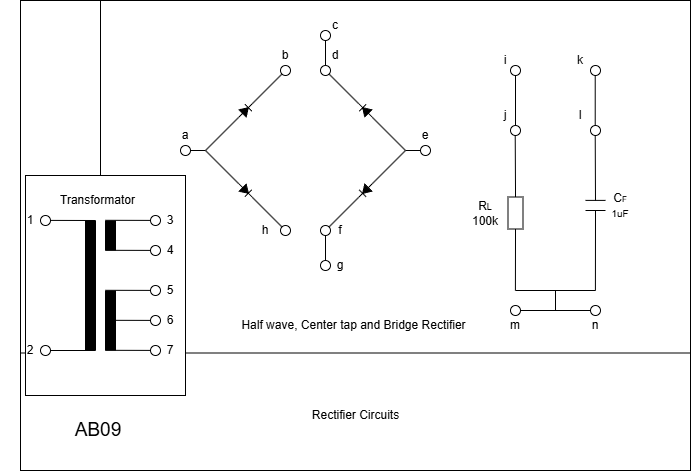
\includegraphics[width=0.8\textwidth]{AB09.png}
    \caption{Schemat obwodu - moduł AB09.}
    \label{fig:schemat}
\end{figure}
\begin{figure}[h]
    \centering
    \includegraphics[width=0.8\textwidth]{1.png}
    \caption{Odczyt z oscyloskopu - wejście.}
    \label{fig:schemat}
\end{figure}
\section*{2.1 Prostownik jednopołówkowy}
Prostownik jednopołówkowy to rzeczywiście najprostsza konfiguracja prostownika, która służy do przekształcania napięcia przemiennego (AC) na napięcie pulsujące stałe (DC). Jego działanie opiera się na wykorzystaniu zaledwie jednej diody półprzewodnikowej, która działa jak jednokierunkowy zawór dla prądu elektrycznego.
\begin{figure}[h]
    \centering
    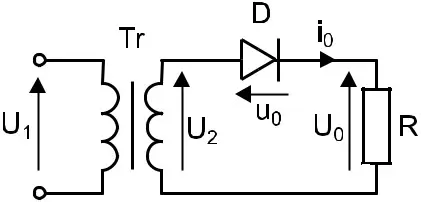
\includegraphics[width=0.8\textwidth]{2.png}
    \caption{Schemat prostownika jednopołówkowego.}
    \label{fig:schemat}
\end{figure}
\section*{Wyniki i obliczenia}

\subsection*{Pomiar}


\begin{itemize}
    \item \textbf{Bez kondensatora:} zakres napięcia: 0 -- 900 mV
    \item \textbf{Z kondensatorem:} napięcie stabilizowane w zakresie 680 -- 840 mV
\end{itemize}
\begin{figure}[h]
    \centering
    \begin{subfigure}{0.45\textwidth}
        \centering
        \includegraphics[width=\linewidth]{3.png}
        \caption{Odczyt pomiaru bez kondensatora.}
        \label{fig:schemat1}
    \end{subfigure}
    \hfill
    \begin{subfigure}{0.45\textwidth}
        \centering
        \includegraphics[width=\linewidth]{4.png}
        \caption{Odczyt pomiaru z kondensatorem.}
        \label{fig:schemat2}
    \end{subfigure}
    \caption{Porównanie odczytów z oraz bez kondensatora.}
    \label{fig:porownanie}
\end{figure}

\subsection*{Teoretyczne obliczenia}

\textbf{Maksymalne napięcie po prostowaniu:}

\[
V_{\text{szczyt}} = V_m - V_D = 2{,}5\,\text{V} - 0{,}7\,\text{V} = 1{,}8\,\text{V}
\]
\textbf{Oznaczenia:}

\begin{itemize}
    \item $V_m$ – amplituda napięcia wejściowego (czyli maksymalna wartość sinusoidy: \SI{2.5}{\volt}),
    \item $V_D$ – spadek napięcia na przewodzącej diodzie (około \SI{0.7}{\volt} dla diody krzemowej).
\end{itemize}

\textbf{Uśrednione napięcie (bez kondensatora):}

\[
V_{dc} = \frac{V_m- V_D}{\pi}  \approx \frac{2{,}5- 0{,}7}{\pi}  \approx \frac{1{,}8}{\pi} = 0{,}573\,\text{V}
\]


\textbf{Sprawność prostownika}

Sprawność prostownika definiujemy jako:

\[
\eta = \left( \frac{V_{dc}}{V_{rms}} \right)^2
\]

\textbf{Gdzie:}

\begin{itemize}
    \item $V_{dc}$ – napięcie średnie na wyjściu,
    \item $V_{rms}$ – wartość skuteczna napięcia wejściowego.
\end{itemize}

\textbf{Obliczenie:}

Przybliżone napięcie średnie (z kondensatorem):

\[
V_{dc} \approx 0.75\,\text{V}
\]

Wartość skuteczna napięcia wejściowego dla sinusoidy o amplitudzie $V_m = 2.5\,\text{V}$:

\[
V_{rms} = \frac{V_m}{\sqrt{2}} = \frac{2.5}{\sqrt{2}} \approx 1.77\,\text{V}
\]

Obliczona sprawność:

\[
\eta = \left( \frac{0.75}{1.77} \right)^2 \approx 0.179 \approx 18\%
\]

\[
\eta = \left(\frac{0{,}75}{1{,}77}\right)^2 \approx 18\%
\]
\section*{2.2 Prostownik dwupołówkowy z odczepem środkowym}

Prostownik dwupołówkowy z odczepem środkowym wykorzystuje dwie diody i transformator z odczepem środkowym. Umożliwia to przewodzenie prądu w obu połówkach cyklu napięcia przemiennego, co skutkuje mniejszymi tętnieniami i wyższą sprawnością w porównaniu z prostownikiem jednopołówkowym.

\begin{figure}[H]
    \centering
    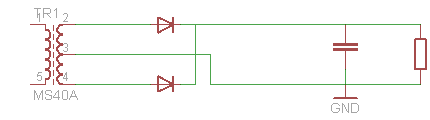
\includegraphics[width=0.8\textwidth]{5.png}
    \caption{Schemat prostownika dwupołówkowego z odczepem środkowym.}
    \label{fig:schemat_dwu}
\end{figure}

\section*{Wyniki i obliczenia}

\subsection*{Pomiar}

\begin{itemize}
    \item \textbf{Bez kondensatora:} napięcie wyjściowe: 0 -- 832 mV
    \item \textbf{Z kondensatorem:} napięcie: 696 -- 784 mV
\end{itemize}
\begin{figure}[h]
    \centering
    \begin{subfigure}{0.45\textwidth}
        \centering
        \includegraphics[width=\linewidth]{6.png}
        \caption{Odczyt pomiaru bez kondensatora.}
        \label{fig:schemat1}
    \end{subfigure}
    \hfill
    \begin{subfigure}{0.45\textwidth}
        \centering
        \includegraphics[width=\linewidth]{7.png}
        \caption{Odczyt pomiaru z kondensatorem.}
        \label{fig:schemat2}
    \end{subfigure}
    \caption{Porównanie odczytów z oraz bez kondensatora.}
    \label{fig:porownanie}
\end{figure}
\subsection*{Teoretyczne obliczenia}

\textbf{Napięcie szczytowe:}

\[
V_{\text{szczyt}} = V_m - V_D = 2{,}5\,\text{V} - 0{,}7\,\text{V} = 1{,}8\,\text{V}
\]

\textbf{Uśrednione napięcie (bez kondensatora):}

\[
V_{dc} \approx \frac{ V_m- V_D}{\pi}  \approx \frac{2{,}5-0{,}7}{\pi} \approx  0{,}57\,\text{V}
\]

\textbf{Sprawność prostownika:}

\[
\eta = \left( \frac{V_{dc}}{V_{rms}} \right)^2
\]

\textbf{Gdzie:}

\begin{itemize}
    \item $V_{dc}$ – napięcie średnie na wyjściu,
    \item $V_{rms}$ – wartość skuteczna napięcia wejściowego.
\end{itemize}

\textbf{Obliczenie:}

\[
V_{dc} \approx 0{,}74\,\text{V}
\]

\[
V_{rms} = \frac{V_m}{\sqrt{2}} = \frac{2{,}5}{\sqrt{2}} \approx 1{,}77\,\text{V}
\]

\[
\eta = \left( \frac{0{,}74}{1{,}77} \right)^2 \approx 0{,}175 \approx 17{,}5\%
\]
\section*{2.3 Prostownik mostkowy (Graetza)}

Prostownik mostkowy, znany również jako układ Graetza, składa się z czterech diod połączonych w mostek. Dzięki temu podczas każdej połówki cyklu napięcia przemiennego prąd płynie przez dwie przewodzące diody, co pozwala uzyskać napięcie wyjściowe o tym samym znaku w obu połówkach cyklu.

\begin{figure}[H]
    \centering
    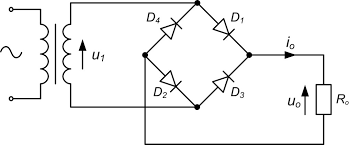
\includegraphics[width=0.8\textwidth]{8.png}
    \caption{Schemat prostownika mostkowego (Graetza).}
    \label{fig:schemat_mostek}
\end{figure}

\section*{Wyniki i obliczenia}

\subsection*{Pomiar}

\begin{itemize}
    \item \textbf{Bez kondensatora:} napięcie wyjściowe: 0 -- 504 mV
    \item \textbf{Z kondensatorem:} napięcie: 352 -- 400 mV
\end{itemize}
\begin{figure}[h]
    \centering
    \begin{subfigure}{0.45\textwidth}
        \centering
        \includegraphics[width=\linewidth]{9.png}
        \caption{Odczyt pomiaru bez kondensatora.}
        \label{fig:schemat1}
    \end{subfigure}
    \hfill
    \begin{subfigure}{0.45\textwidth}
        \centering
        \includegraphics[width=\linewidth]{10.png}
        \caption{Odczyt pomiaru z kondensatorem.}
        \label{fig:schemat2}
    \end{subfigure}
    \caption{Porównanie odczytów z oraz bez kondensatora.}
    \label{fig:porownanie}
\end{figure}

\subsection*{Teoretyczne obliczenia}

\textbf{Napięcie szczytowe (dwie diody przewodzą):}

\[
V_{\text{szczyt}} = V_m - 2V_D = 2{,}5\,\text{V} - 1{,}4\,\text{V} = 1{,}1\,\text{V}
\]

\textbf{Uśrednione napięcie:}

\[
V_{dc} = \frac{2 V_m}{\pi} - 2 V_D \approx \frac{5}{\pi} - 1{,}4 \approx 1{,}59 - 1{,}4 = 0{,}19\,\text{V}
\]

\textbf{Sprawność prostownika:}

\[
\eta = \left( \frac{V_{dc}}{V_{rms}} \right)^2
\]

\textbf{Gdzie:}

\begin{itemize}
    \item $V_{dc}$ – napięcie średnie na wyjściu,
    \item $V_{rms}$ – wartość skuteczna napięcia wejściowego.
\end{itemize}

\textbf{Obliczenie:}

\[
V_{dc} \approx 0{,}380\,\text{V}
\]

\[
V_{rms} = \frac{V_m}{\sqrt{2}} = \frac{2{,}5}{\sqrt{2}} \approx 1{,}77\,\text{V}
\]

\[
\eta = \left( \frac{0{,}380}{1{,}77} \right)^2 \approx 0{,}045 \approx 4{,}5\%
\]
\section*{3. Dyskusja błędów}

Podczas pomiarów mogły wystąpić różne błędy, które wpłynęły na wyniki. Przede wszystkim używany oscyloskop mógł nie pokazywać dokładnych wartości napięcia średniego, zwłaszcza gdy napięcie zmieniało się szybko lub było impulsowe. Spadek napięcia na diodach mógł się różnić od typowego 0,7 V, ponieważ prąd był bardzo mały ze względu na dużą rezystancję obciążenia. Dodatkowo warto zauważyć, że badania były prowadzone przy małym napięciu wejściowym (około 2,5 V szczytowego), więc spadek 0,7 V na diodzie to stosunkowo duża strata – co mocno wpływało na wyniki. Napięcie z generatora mogło też nie być idealnie sinusoidalne.
Możliwe były również błędy przy ręcznym odczycie i zapisie wyników, szczególnie jeśli wskazania były niestabilne. Wpływ mogły mieć też niedokładności elementów w układzie, takie jak tolerancja rezystorów czy różnice między diodami. Pomiar z kondensatorem również mógł być mniej precyzyjny, bo napięcie na wyjściu nie było całkowicie stałe.

\section*{4. Wnioski}

Podczas ćwiczenia zbadaliśmy działanie trzech rodzajów prostowników: jednopołówkowego, dwupołówkowego z odczepem środkowym oraz mostkowego. Otrzymane przebiegi i napięcia średnie były zbliżone do ogólnych oczekiwań teoretycznych, co potwierdziło poprawność działania układów. Największe napięcie średnie uzyskaliśmy w prostowniku dwupołówkowym, a najmniejsze w jednopołówkowym, co zgadza się z teorią. Zauważyliśmy również, że kondensator znacznie poprawiał przebieg napięcia wyjściowego, zmniejszając tętnienia.

Spadki napięcia na diodach miały duży wpływ na wyniki, ponieważ przy niskim napięciu wejściowym (ok. 2,5 V) strata 0,7 V była znacząca. W prostowniku mostkowym, gdzie napięcie spada na dwóch diodach jednocześnie, efekt ten był jeszcze silniejszy. Zaobserwowaliśmy dużą różnicę między teoretyczną maksymalną sprawnością a sprawnością uzyskaną w praktyce. Prawdopodobną przyczyną był bardzo mały prąd w układzie, który powodował duży relatywny wpływ spadków napięcia na diodach.

Drobne różnice w wynikach mogły być również spowodowane niedokładnością pomiarów oraz tolerancją użytych elementów. Ogólnie uzyskane wyniki potwierdziły działanie prostowników zgodnie z przewidywaniami, choć widoczne były praktyczne ograniczenia układów przy pracy z niskim napięciem i małym obciążeniem.

\end{document}
